\documentclass{sigchi}

%% EXAMPLE BEGIN -- HOW TO OVERRIDE THE DEFAULT COPYRIGHT STRIP -- (July 22, 2013 - Paul Baumann)
\toappear{}
%% EXAMPLE END -- HOW TO OVERRIDE THE DEFAULT COPYRIGHT STRIP -- (July 22, 2013 - Paul Baumann)

\pagenumbering{arabic}

% Load basic packages
\usepackage{balance}  % to better equalize the last page
\usepackage{graphics} % for EPS, load graphicx instead 
\usepackage[T1]{fontenc}
\usepackage{txfonts}
\usepackage{mathptmx}
\usepackage[pdftex]{hyperref}
\usepackage{color}
\usepackage{booktabs}
\usepackage{textcomp}
% Some optional stuff you might like/need.
\usepackage{microtype} % Improved Tracking and Kerning
% \usepackage[all]{hypcap}  % Fixes bug in hyperref caption linking
\usepackage{ccicons}  % Cite your images correctly!
\usepackage[utf8]{inputenc} % for a UTF8 editor only
\usepackage[ngerman]{babel}

% If you want to use todo notes, marginpars etc. during creation of your draft document, you
% have to enable the "chi_draft" option for the document class. To do this, change the very first
% line to: "\documentclass[chi_draft]{sigchi}". You can then place todo notes by using the "\todo{...}"
% command. Make sure to disable the draft option again before submitting your final document.
\usepackage{todonotes}

% Paper metadata (use plain text, for PDF inclusion and later
% re-using, if desired).  Use \emtpyauthor when submitting for review
% so you remain anonymous.
\def\plaintitle{Lock-a-dos: Ein Rucksack mit Selbstschutz}
\def\plainauthor{Alexander Schuhmann, Maximilian Balluff, Michael Stadler, Maximilian Pachl}
\def\emptyauthor{}
\def\plainkeywords{Rucksack; Diebstahl; Selbstüberwachung; Smartphone; Sensoren; Wearable}
\def\plaingeneralterms{Dokumentation}

% llt: Define a global style for URLs, rather that the default one
\makeatletter
\def\url@leostyle{%
  \@ifundefined{selectfont}{
    \def\UrlFont{\sf}
  }{
    \def\UrlFont{\small\bf\ttfamily}
  }}
\makeatother
\urlstyle{leo}

% To make various LaTeX processors do the right thing with page size.
\def\pprw{8.5in}
\def\pprh{11in}
\special{papersize=\pprw,\pprh}
\setlength{\paperwidth}{\pprw}
\setlength{\paperheight}{\pprh}
\setlength{\pdfpagewidth}{\pprw}
\setlength{\pdfpageheight}{\pprh}

% Make sure hyperref comes last of your loaded packages, to give it a
% fighting chance of not being over-written, since its job is to
% redefine many LaTeX commands.
\definecolor{linkColor}{RGB}{6,125,233}
\hypersetup{%
  pdftitle={\plaintitle},
% Use \plainauthor for final version.
%  pdfauthor={\plainauthor},
  pdfauthor={\emptyauthor},
  pdfkeywords={\plainkeywords},
  bookmarksnumbered,
  pdfstartview={FitH},
  colorlinks,
  citecolor=black,
  filecolor=black,
  linkcolor=black,
  urlcolor=linkColor,
  breaklinks=true,
}

% create a shortcut to typeset table headings
% \newcommand\tabhead[1]{\small\textbf{#1}}

% End of preamble. Here it comes the document.
\begin{document}

\title{\plaintitle}

\numberofauthors{4}
\author{%
  \alignauthor{Alexander Schuhmann\\
    \email{e-mail address}}\\
  \alignauthor{Maximilian Balluff\\
    \email{e-mail address}}\\
  \alignauthor{Michael Stadler\\
    \email{e-mail address}}\\
  \alignauthor{Maximilian Pachl\\
    \email{pachl@hm.edu}}\\
}

\maketitle

\begin{abstract}
  Aktualisiert---\today. Dieses Paper beschreibt die prototypische
  Umsetzung eines Rucksacks, der sich selbst vor dem Zugriff Dritter
  schützen kann. Dazu werden eine Reihe von Sensoren in den Rucksack
  integriert um mögliche Einflüsse von Außen jederzeit erkennen zu
  können. Ein Alarm sorgt dafür, dass der unbefugte Zugriff nicht
  unbemerkt bleibt. Mithilfe eines Smartphones kann der Besitzer
  die Selbstüberwachung des Rucksackes ein- und ausschalten.
\end{abstract}

\subsection{Schlagwörter}
\plainkeywords

\section{Einleitung}
Manchmal ist es gar nicht so leicht alleine mit seinem Gepäck
unterwegs zu sein. Beispielweise möchte man seine Sachen nicht 
unbeaufsichtigt am Strand zurücklassen, wenn man eine Runde
im Meer schwimmen möchte. Gerade in beliebten Urlaubsregionen
kommt es schnell mal vor, dass man um seinen Geldbeutel 
erleichtert wird. Um diesem Problem vorzubeugen wurde im Rahmen
dieser Arbeit ein Rucksack entwickelt, der durch eine vielzahl
von Sensoren erkennen kann ob sich jemand an dem gesicherten
Rucksack zu schaffen macht. Zusätzlich wird mit einem
elektronischen Schloss das Hauptfach zugesperrt. Im Falle eines
unberechtigten Zugriffes sind mehrere Abwehrmechanismen denkbar:

\begin{itemize} 
\item Lauter Alarm zur Abschreckung
\item SMS an Besitzer mit GPS Position
\item Stromschläge durch einen Taser
\end{itemize}

Zur komfortablen Konfiguration kann der Besitzer mit seinem
Smartphone verschiedene Profile für verschiedene Situationen 
(Bsp.: Beschleunigungssensor ignorieren, wenn auf dem Rücken getragen)
erstellen und aktivieren. Bei der vorliegenden Umsetzung handelt
es sich nur um einen Prototypen der weder auf Kosten, noch auf
Platzverbrauch optimiert ist.

\section{Plattform}
Als Entwicklungsplattform wurde ein RaspberryPi eingesetzt. Dabei
handelt es sich um einen sehr kleinen Einplatinencomputer, der
über diverse Ein- und Ausgangsschnittstellen verfügt und ein
Debian Linux als Betriebssystem ausführt. Da es für das RaspberryPi
eine sehr große Community gibt eignet es sich sehr gut als
Prototying Plattform. Dank des standard Linuxsystems kann 
jede bliebige Hochsprache zur Implementierung der Software
verwendet werden. Die Software wurde ausschließlich in Python
umgesetzt und kann unter \cite{Github:Software} abgerufen werden.

\subsection{Hotspot}

\subsection{Webapplikation}

\section{Sensorik}

\subsection{Thermosensor}

\subsection{Beschleunigungssensor}
Um detektieren zu können ob der Rucksack in Bewegung ist oder
still steht wird ein Beschleunigungssensor verwendet. Dieser
Sensor fertigt ein Akzelerogramm an. Das bedeutet, dass die
Geschwindigkeitszu- und abnahme kontinuierlich überwacht wird.
Dabei werden alle drei Raumachsen (X, Y u. Z) separat aufgezeichnet.
Wenn der Rucksack nun ruckartig vom Boden aufgehoben wird, erfährt er
eine Beschleunigung in Z-Richtung. Diese Abweichung vom
Normalzustand kann in der Auswertesoftware detektiert werden
und je nach Konfiguration zu einem Alarm führen. Dabei wird 
eine einfache Schwellwertfilterung auf den Sensor angewendet.
Um Bewegungen in alle Richtungen erkennen zu können werden natürlich
auch die aderen Raumachsen mit ausgeweretet.

\begin{figure}
\centering
  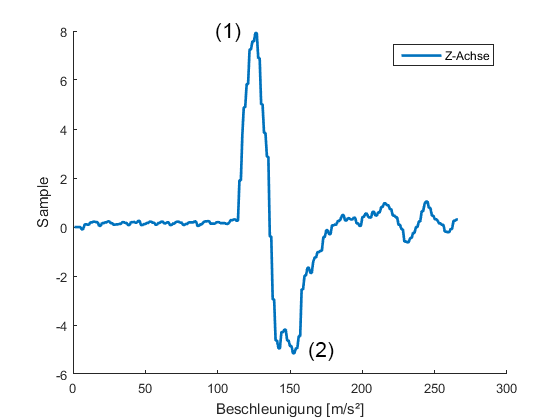
\includegraphics[width=0.9\columnwidth]{fig/accel_z.png}
  \caption{Akzelerogramm der Z-Achse beim Aufheben des Rucksacks}
  \label{fig:accel_z}
\end{figure}

Abbildung \ref{fig:accel_z} zeigt ein Akzelerogramm der Z-Achse,
das beim Aufheben des Rucksacks aufgezeichnet wurde. Der Peak (1)
in positiver Y-Richtung zeigt die Beschleunigung des Rucksackes
beim Aufheben an. Der Peak (2) in negativer Richtung zeigt das
Abremsen des Rucksacks an wenn die Aufhebebewegung abgeschlossen
ist. Der zu verwendende Schwellwert wurde in einer kleinen
Versuchsreihe expirementell bestimmt. Ein Schwellwert von \textit{1}
hat sich dabei als guter Wert herausgestellt. Dadurch kann
Sensorrauschen von einer tatsächlichen Bewegung unterschieden
werden. Der Erkennungsalgorithmus schlägt nur Alarm, wenn mehr
wie drei konsekutive Messungen über dem Schwellwert liegen. Damit
soll vermieden werden, dass Fehlmessungen einen Alarm auslösen.
Bei der Umsetzung des Prototypen wurde der BNO055 \cite{Bosch:BNO055}
von Bosch als Sensorsystem verwendet. Dieser wird im UART Modus
betrieben und über einen USB-TTL Adapter an das RaspberryPi
angebunden. Der Schritt über den USB Adapter ist nötig, da der
interne UART bereits für den GPS Empfänger verwendet wird.

\subsection{Lichtsensor}

\subsection{GPS}

\section{Aktoren}

\subsection{Elektronisches Schloss}

\subsection{Alarm}

\section{Fazit}

\balance{}

% REFERENCES FORMAT
% References must be the same font size as other body text.
\bibliographystyle{SIGCHI-Reference-Format}
\bibliography{main}

\end{document}
